\begin{comment}
Analysieren der Suchabfragen
\begin{itemize}
    \item Testdaten bestimmen.
    \item Qualität der Suche anhand von Precison und Recall mit den Testdaten bestimmen.
\end{itemize}


\paragraph{Result} \hfill \\
\begin{itemize}
    \item Definition von Beispiel-Anfragen und den dazu erwarteten Antworten.
    \item Analyse der Resultate.
\end{itemize}
\end{comment}


\chapter{Analyse der Abfrage}
\label{ch:analysis}

Um dieses Information Retrieval System zu bewerten,
möchten wir die Precision (Genaugkeit) und den Recall
(Trefferquote) für typische Abfragen an das System
bestimmen. Um die dazu notwendigen Daten zu erheben
verwenden wir das Entwicklungs und Analyse
Tool für Lucene Indizes Luke.

\paragraph{Luke} kann unter anderem verwendet werden um Dokumente
im Index zu betrachten (\cref{fig:luke-docs}) oder
um Abfragen zu erstellen (\cref{fig:luke-search}).
\cite{web:lukeintro}
Luke \cite{web:luke} scheint vom ursprünglichen
Entwickler \citeauthor{web:luke}
nicht mehr maintained zu werden. Von \citeauthor{web:lukegit}
ist eine Version verfügbar in welcher auch Indizes
von Lucene in der aktuellen Version gelesen werden
können. \cite{web:lukegit}

\begin{figure}[h]
    \centering
    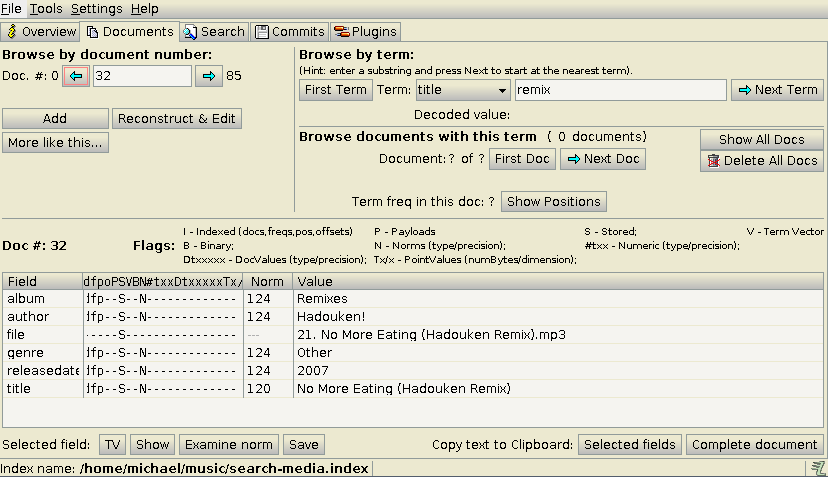
\includegraphics[width=\textwidth]{luke-documents}
    \caption{Ansicht Dokumente in Luke}
    \label{fig:luke-docs}
\end{figure}

\begin{figure}[h]
    \centering
    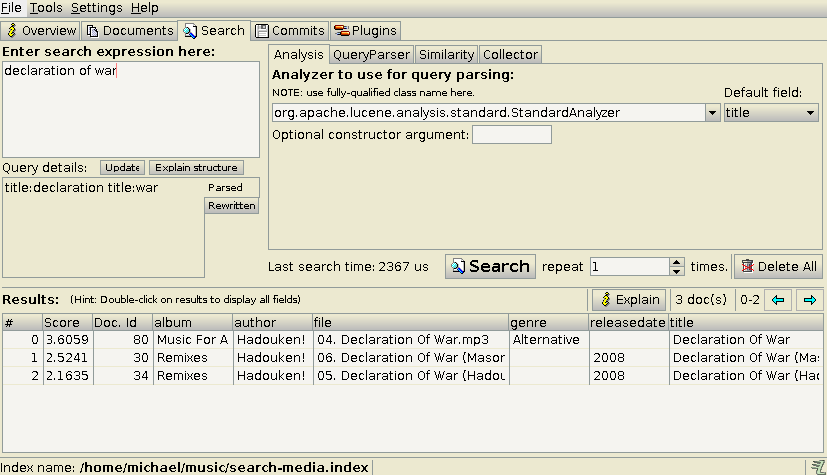
\includegraphics[width=\textwidth]{luke-search}
    \caption{Ansicht Suche in Luke}
    \label{fig:luke-search}
\end{figure}

\section{Test Daten}
\label{sec:testdata}
Damit man eine verlässliche Aussage über die Precision
und den Recall machen kann, muss man die indizierten
Dokumente genau kennen. Das heisst wir müssen genau
wissen welches die erwarteten Treffer einer Abfrage
sind.\cite[S.~152]{book:manning}

Aus der Media Library wählen wir dazu eine Menge
von \(85\) Dateien aus und erstellen einen Index,
worin nur diese Dateien indiziert werden.

\begin{table}[h]
    \centering
    \begin{tabu}{l|c}
        \hline
        \rowfont[c]{\bfseries} Abfrage & \#Resultat \\
        \hline
        *:*                               & \(85\) \\
        author:hadouken                   & \(66\) \\
        author:hadouken AND title:war     & \(3\) \\
        author:hadouken AND NOT title:war & \(63\) \\
        title:girl*                       & \(4\) \\
        title:liquid AND releasedate:2007 & \(4\) \\
        album:"museums of consciousness"  & \(7\)
    \end{tabu}
    \caption{Abfragen und Erwartete Resultate}
    \label{tab:testdata}
\end{table}

Mit den Abfragen in \cref{tab:testdata}, wollen wir ein
Spektrum von Abfragen abdecken, welches nahe am tatsächlichen
Gebrauch eines solchen Index ist. Die Anzahl
der erwarteten Results wird mit EasyTAG gezählt,
es werden dazu nicht die Dokumente in Luke betrachtet.
Damit würden allfällige Fehler, welche beim Indizieren
oder beim Abfragen mit Luke entstehen könnten,
kaschiert.


\section{Precision \& Recall}
Die vorbereiteten Abfragen führen wir nun mit Luke aus.
Von den die erhaltenen Resultate vergleichen wir dann
mit den gespeicherten Resultaten der in \cref{sec:testdata}
vorbereiteten Abfragen.

Seien \(e\) die erwarteten Resultate und \(r\)
das erreichte Resultat. Dann sind die Precision und
dre Recall wie folgt definiert.

\begin{description}
    \item [Recall] Die Fähigkeit die erwarteten Resultate zu liefern. \(r = \frac{|r \cap e|}{|e|}\)
    \item [Precision] Die Korrektheit der gelieferten Resultate. \(p = \frac{|r \cap e|}{|r|}\)
\end{description} \cite[S.~63]{book:heinrich}

\begin{table}[h]
    \centering
    \begin{tabu}{l|c|c|c|c|c}
        \hline
        \rowfont[c]{\bfseries} Abfrage & \(|r|\) & \(|e|\) & \(|r \cap e|\) & \(p\) & \(r\) \\
        \hline
        *:*                               & \(85\) & \(85\) & \(85\) & \(1\) & \(1\) \\
        author:hadouken                   & \(66\) & \(66\) & \(66\) & \(1\) & \(1\) \\
        author:hadouken AND title:war     & \(3\)  & \(3\)  & \(3\)  & \(1\) & \(1\) \\
        author:hadouken AND NOT title:war & \(63\) & \(63\) & \(63\) & \(1\) & \(1\) \\
        title:girl*                       & \(4\)  & \(4\)  & \(4\)  & \(1\) & \(1\) \\
        title:liquid AND releasedate:2007 & \(4\)  & \(4\)  & \(4\)  & \(1\) & \(1\) \\
        album:"museums of consciousness" \footnotemark  & \(0\)  & \(7\)  & \(0\)  & \(-\) & \(0\)
    \end{tabu}
    \caption{Abfragen und Erreichte Resultate}
    \label{tab:testresult}
\end{table}
\footnotetext{Diese Abfrage muss mit dem Luke XML Query Parser ausgeführt werden, in regulären Abfragen entfernt Luke \emph{of} aus dem String, so dass nur noch nach album:"museums consciousness" gesucht wird.}

Diese Resultate scheinen im ersten Moment etwas überraschend,
lassen sich jedoch erklären. Bis auf die letzte Zeile sind
jeweils genau die erwarteten Resultate erreicht worden. Dafür
gibt es unterschiedliche Gründe. Die Menge ist relativ klein,
die Wahrscheinlichkeit sinkt dadurch Ausreisser zu treffen.
Die Abfragen sind einfach, es wurden keine N-Gramme geladen,
es existieren keine Ähnlichkeitsabfragen. Dies alles sind
Features welche eine Suche in verschiedenen Bereichen für
einen Endanwender bequemer jedoch auch ungenauer  machen.

Dann ist in diesem noch das Resultate, bei welchem kein Hit
gefunden wurde. Dies liegt an der String Suche, in
\cref{sec:createindex} haben wir die meisten Attribute des
Dokuments, darunter auch \emph{album}, als \emph{TextField} 
erstellt. Ein \emph{TextField} wird in einzelne Worte aufgeteilt,
davon werden nur die einzelnen Worte indiziert, nicht der
gesamte String. Um auf diesem Feld auch eine String
Suche zu ermöglichen, könnte als mögliche Lösung ein
zusätzliches \emph{StringField} mit dem gesamten String zum Dokument
hinzugefügt werden. Dies müsste jedoch nicht auch gespeichert werden.
